\documentclass[../main]{subfiles}
\begin{document}

\section{Environment Configuration}
Configuring your environment can be quite frustrating at times and can eat away a lot of time. For that reason,
here are some instructions for getting you set up quickly. Moreover, it is also helpful to know how to configure a
modelling project. An unorganised project saps away productivity so I also detail here one way of organising your
project, specifically for modelling with PyCoTools, COPASI and tellurium. If you run
into problems, you can clone or fork an example project from \href{https://github.com/CiaranWelsh/ExampleProject}{here}.

It would be helpful if the configuration was done prior to the sessions as then we can focus on modelling
issues, rather than configuration issues.

\subsection{Python}
Python is a program written in C. It is an executable file (i.e. a binary) that must be compiled and linked
from source before you can use it. There are many `distributions' of Python, which essentially just means
different people have compiled it and packaged it in slightly different ways.

My favourite distribution of Python is \href{https://docs.conda.io/en/latest/miniconda.html}{Miniconda}. Miniconda
and Anaconda are essentially the same, but Anaconda comes with a whole bunch of additional Python packages. These
can be useful, but it is quicker to just use Miniconda.

\begin{Task}[label=InstallMiniconda]{Install Miniconda}
Google Miniconda and follow the instructions to install Miniconda.
\end{Task}

\warning{Make sure the command `conda` works from terminal or cmd. If it doesn't then you
need to add the Miniconda bin directory to your path environment variable}

Anaconda and Miniconda (or just Conda) allows you to create isolated Python environments
and switch between them easily. Think of each conda environment you have as a box that is
kept separate from the other Python `boxes'. While the full documentation can be found \href{https://docs.conda.io/projects/conda/en/latest/user-guide/tasks/manage-environments.html}{here}
the commands to create a conda environment are quite simple.

\begin{minted}{bash}
$ conda create --name py36 python=3.6
\end{minted}

Will create a conda environment.

\begin{minted}{bash}
$ conda activate py36
\end{minted}

will switch to the environment

and

\begin{minted}{bash}
$ pip install pycotools3 tellurium
\end{minted}

will install pycotools3 and tellurium, with all their dependencies.

\warning{Neither pycotools3 or tellurium work on Python 3.7 or 3.8. This is because of a broken dependency. The
issue is in the process of being solved (apparently)}

\subsection{COPASI}

\begin{Task}{Install COPASI}
Install Copasi and configure the environment variables if you need to. You should be able to
run `CopasiUI` from the terminal.
\end{Task}

\subsection{PyCharm}
PyCharm is a significantly better IDE than many of the alternatives. It does a lot for you. You can also
get a free Licence for the Pro edition with your university email address. Learning how to use
PyCharm is useful for many reasons, one of which is that if and when you migrate to other programming
languages, JetBrains will have a an IDE for you. Since all the IDE's are very similar, you only have
to learn to use one and the rest fall in place.

\begin{Task}{Install PyCharm}
Install PyCharm. I prefer to install the JetBrains toolbox and install the IDE from there.
\end{Task}

\subsection{Configuring a Project}
You can configure a project however you like, but with a small amount of effort you can create an
organised Python project. Being organised makes things much easier down the line. We will be creating a
GitHub repository which contains a Python package that has two subpackages, one for models and the other
for data.

A package in Python is marked by the special file called `\_\_init\_\_.py'. Even if it is a black file,
the presence of this file in a directory marks it as a Python directory. Whenever a Package is imported, the
\_\_init\_\_.py (for initialisation) is automatically executed. This makes it a convenient place to store
some global variables that can be used anywhere throughout the project.

Throughput the project, we will be using:
\begin{itemize}
    \item The main \_\_init\_\_.py file (ExampleProject/example\_project/\_\_inti\_\_.py) to hold global variables, such as path names, to be used throughout the project
    \begin{itemize}
        \item \note{The other two \_\_init\_\_.py files will be empty}
    \end{itemize}
    \item The `model' package to hold all data regarding models such as the code for building, estimating the parameters of and simulating a model
    \item The `model\_strings.py' file as a storage module to keep model strings isolated from the execution code
    \item The `control\_script.py' file for containing code for actually running the script
    \item The `data' module for holding everything regarding experimental data, such as raw data files and data analysis scripts
    \item The `data\_analysis.py' script for doing anything data related (normalisation, plotting or automatically formatting for COPASI)
    \item The `CopasiFormattedData` folder to hold all experimental data that is already formatted for COPASI (whether this is done manually or automatically).
\end{itemize}

\begin{Task}{Create a Project}
In PyCharm, create a new project. Then create a directory tree which looks like Figure \ref{fig:config:example_project}.
\end{Task}

A few pieces of code should be added to this project before we begin modelling. Firstly,
we are essentially building a Python package but from within the package we are building. Therefore, When
importing, Python will look for this package in all the usual places and not be able to find it. To overcome
this problem, we can simply tell Python where our project is using the `site' package to add the directory
containing `example\_project' to the Python Path variable.

\note{PyCharm has options in `run configuration` for adding your project directories to the PYTHON\_PATH
variable. These are usually set to True by default, so if you use Pycharm you actually don't need this step.
However, if the code is ported to another IDE (such as Spyder) you may run into problems}


\begin{figure}
\centering
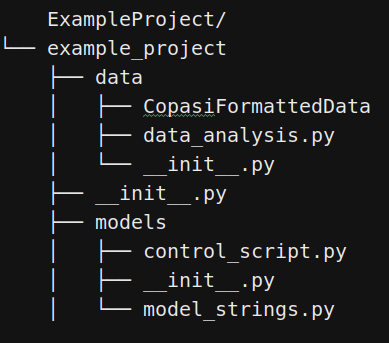
\includegraphics[width=0.4\linewidth]{EnvConfig/assets/example_project_config}
\caption{Directory tree for organised modelling project}
\label{fig:config:example_project}
\end{figure}


\begin{Task}{Configure the PYTHON\_PATH variable}
Inside `ExampleProject/example\_project/models/control\_script.py' put

\begin{minted}{python}
import os
import site
# Add path to sources root to Python's PATH variable
site.addsitedir(os.path.dirname(os.path.dirname(os.path.abspath(''))))
# note: Pycharm already doesn't this for you.
#  But doesn't hurt to add it here anyway

# Go and get the model string by importing it from your models_strings module
from example_project.models.model_strings import model_string

# imports all the global variables (notice that we
#  can print out the WORKING_DIRECTORY variable)
from example_project import *


# Any functions or classes you write will go here

if __name__ == '__main__':

# Any code that uses the functions or classes your have created above,
# will go here. We will be using flags defined in our __init__.py
# to modify the behaviour of this script. Since the Flags are boolean,
# we just us a simple if statement for each of them

if PRINT_WORKING_DIRECTORY:
# prints /home/ncw135/Documents/ExampleProject/example_project
print(WORKING_DIRECTORY)

\end{minted}
\end{Task}

\begin{Task}{Configure the your projects global variables}
Add the following to `ExampleProject/example\_project/\_\_init\_\_.py'.
\begin{minted}{python}
import os, glob
# Global variables are always in caps, to distinguish them from local variables.
WORKING_DIRECTORY = os.path.dirname(__file__)
DATA_DIR = os.path.join(WORKING_DIRECTORY, 'data')
COPASI_FORMATTED_DATA_DIR = os.path.join(DATA_DIR, 'CopasiFormattedData')

# Flags that change the behaviour of the control_script

# flag to demonstrate the principle of flags
PRINT_WORKING_DIRECTORY = True

\end{minted}
\end{Task}

Now, because of our configuration we can import the various parts of the project
within the `control\_script' and begin modelling.

\note{If something isn't working and you've spend too much time trying to fix,
you can clone or fork my example \href{https://github.com/CiaranWelsh/ExampleProject}{project} from Github}.

\begin{Task}{Create a GitHub Repository}
Sign up for a GitHub account if you do not already have one. Turn your version of this bioler plate
project into a GitHub repository. One set of instructions can be found
\href{https://help.github.com/en/github/getting-started-with-github/create-a-repo}{here}.
\end{Task}

\end{document}